\chapter{Entity Triggers}
This section is adapted from the research paper I co-authored titled ``Entity Triggers: Learning with Explanations for Named Entity Recognition'' which will appear in the 2020 Association for Computational Linguistics conference.



\section{Motivation}
%Should I talk about our approach using weak labels first? The weak labels didn't work bc don't know which word trigger refers to
\label{sec:intro}
Recent advances in NER have primarily focused on training neural network models with an abundance of human annotations, yielding state-of-the-art results \citep{LampleNER}. However, NER often requires huge amounts of labeled data (e.g. tens of thousands of labeled sentences). Collecting these human annotations is expensive and time-consuming, especially in technical domains such as biomedical publications, financial documents, legal reports, etc. As we seek to advance NER into more domains with less human effort, how to learn neural models for NER in a annotation-efficient way becomes a crucial research problem.

The standard protocol for obtaining an annotated NER dataset involves an annotator viewing a sentence, selecting token spans as entities, and labeling the spans with their entity types. Because this annotation process provides limited supervision per example, in order to train a high-performance model, it is necessary to collect a large amount of annotations. Given the effort the annotator has already spent analysing the sentence and recognizing the entity, we aim to investigate how we can obtain extra supervision from this entity annotation.

A human's recognition of an unlabeled entity usually depends on cue words or  phrases in the sentence. For instance, we cold infer that the randomized word \underline{Kasdfrcxzv} is likely to be a location entity mention in the sentence ``Tom \textit{traveled} a lot last year \textit{in} \underline{Kasdfrcxzv}.'' We recognize this location entity because of the cue phrase ``\textit{travel} ... \textit{in},'' which indicates that there should be a location entity after the word ``\textit{in}.'' We hypothesize that these cue phrases not only explain the recognition process, but can also help our NER models to learn and generalize faster. We call such entity-associated rational phrases \textit{entity triggers}. Specifically, we define an entity trigger (or trigger for simplicity) as a group of words that can help explain the recognition process of a particular entity in the same sentence. For example, in~\figref{fig:trigex}, \textit{``had ... lunch at''}\footnote{Note that a trigger can be a discontinuous phrase.} and \textit{``where the food''} are two distinct triggers associated with the \textsc{Restaurant} entity ``\underline{Rumble Fish}.'' An entity trigger should be a necessary and sufficient cue for humans to recognize its associated entity even if we mask the entity with a random word. Thus, unnecessary words such as ``fantastic'' should not be  considered part of the entity trigger.

\begin{figure}[h]
	\centering
	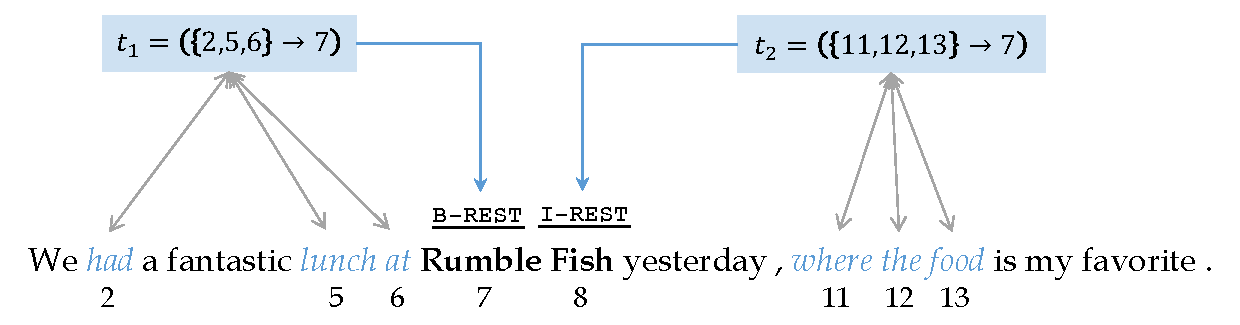
\includegraphics[width=0.85\linewidth]{LatexDiss/figures/trigexample.pdf}
	\caption{Example of entity triggers: \textit{``had(2) ... lunch(5) at(6)''} and \textit{``where(11) the(12) food(13)''} are two individual entity triggers associated to the entity mention {\underline{``Rumble Fish''}} typed as \texttt{REST}aurant, which starts at the 7th token.}
	\label{fig:trigex}
\end{figure}

We argue the benefits of supervising models using a combination of entity triggers and standard entity annotations. This approach is more powerful because unlabeled sentences, such as ``Bill \textit{enjoyed} a great \textit{dinner} with Alice \textit{at} \underline{Zcxlbz}.'' can be matched with the existing trigger ``\textit{had} ... \textit{lunch at}'' via their semantic relatedness. This makes it easier for NER models to recognize \underline{Zcxlbz} as a \textsc{Restaurant} entity than if we had only trained the NER model using entity labels. In contrast, if we only had the entity annotation itself (i.e. ``\underline{Rumble Fish}'') as supervision, the model would require many similar examples in order to learn this simple pattern. Annotating triggers in addition to entities is not significantly more laborious since annotators have already read the sentences and analysed the entities. Thus, we hypothesize that using triggers as additional supervision is a more cost-effective way to train models.

We crowd-sourced 14,708 triggers on two well-studied NER datasets to study the usefulness of entity triggers. We proposed a novel framework named \textit{Trigger Matching Network} ({TMN}). Because it exploits triggers, TMN is more powerful and cost-effective than standard approaches. The TMN framework consists of three components: 1) a trigger encoder, 2) a semantic trigger matching module, and 3) an entity tagger. Our first learning stage jointly trains the trigger encoder and semantic trigger matching module. We then learn a sequence tagger using trigger-enhanced attentions in order to incorporate existing trigger information into entity predictions on unseen sentences.

Our contributions are as follows:
\begin{itemize}
    \item We introduced the concept of ``entity triggers,'' a novel form of explanatory annotation for named entity recognition problems.  We crowd-sourced and publicly released 14k annotated entity triggers on two popular datasets: \textit{CoNLL03} (generic domain), \textit{BC5DR} (biomedical domain).
    \item We proposed a novel learning framework, named \textit{Trigger Matching Network}, which encodes entity triggers and softly grounds them on unlabeled sentences to increase the effectiveness of the base entity tagger (Section~\ref{sec:tmn}). 
    \item Experimental results (Section~\ref{sec:exp}) show that the proposed trigger-based framework is significantly more cost-effective. The TMN only uses 20\% of the trigger-annotated sentences from the original CoNLL03 dataset and achieves comparable performance to the conventional model using 70\% of the annotated sentences. 
\end{itemize}





\section{Problem Formulation}
\label{sec:problem}
We consider the problem of how to cost-effectively learn a model for NER using entity triggers. This section introduces basic notations and provides a formal task definition for learning using entity triggers.

In the conventional setup for supervised learning for NER, we let $\mathbf{x}=[x^{(1)}, x^{(2)}, \cdots, x^{(n)}]$ denote a sentence in the labeled training corpus $\mathcal{D}_{L}$.
Each labeled sentence has a NER-tag sequence $\textbf{y}=[y^{(1)}, y^{(2)}, \cdots, y^{(n)}]$, where $y^{(i)}\in \mathcal{Y}$ and  $\mathcal{Y}$ can be \{\texttt{O}, \texttt{B-PER}, \texttt{I-PER}, \texttt{B-LOC}, \texttt{I-LOC}, $\cdots$\}. Here, \texttt{O} represents a non-entity, \texttt{B-TYPE} represents the beginning of an entity of type \texttt{TYPE} and \texttt{I-TYPE} remaining words in an entity. The possible tags come from a BIO or BIOES tagging schema for segmenting and typing entity tokens.
Thus, we have $\mathcal{D}_{L}=\{(\mathbf{x_i}, \mathbf{y_i})\}$, and an unlabeled corpus $\mathcal{D}_{U}=\{\mathbf{x_i}\}$ that we want to label.

We use $T(\mathbf{x},\mathbf{y})$ to represent the set of annotated entity triggers, where each trigger $t_i\in T(\mathbf{x},\mathbf{y})$ is associated with an entity index $e$ and a set of word indices $\{w_i\}$.
Note that we use the index of the first word of an entity as its entity index.
That is, $t = (\{w_1, w_2, \cdots\}\rightarrow{e})$, where $e$ and $w_i$ are integers in the range of $[1,|\mathbf{x}|]$. \quad
For instance, in the example shown in Figure~\ref{fig:trigex}, the trigger \textit{``had ... lunch at''} can be represented as a trigger $t_1=(\{2,5,6\}\rightarrow{7})$, because this trigger specifies the entity starting at index $7$, \textit{``Rumble''}, and it contains a set of words with indices: \textit{``had''} ($2$), \textit{``lunch''} ($5$), and \textit{``at''} ($6$).
Similarly, we can represent the second trigger \textit{``where the food''} as $t_2 = (\{11,12,13\}\rightarrow{7})$.
Thus, we have $T(\mathbf{x},\mathbf{y})=\{t_1, t_2\}$ for this sentence.

Adding triggers creates a new form of data $\mathcal{D}_{T} = \{(\mathbf{x_i},\mathbf{y_i}, T(\mathbf{x_i},\mathbf{y_i})\}$. 
Our goal in this paper is to learn a model for NER from a trigger-labeled dataset $\mathcal{D}_T$, such that we can achieve comparable learning performance to a mdoel using a much larger $\mathcal{D}_L$.





\section{Proposed Framework}
\label{sec:tmn}
This section presents our framework for a more cost-effective learning method for NER using triggers. Our intuition is to treat triggers as soft templates such that new sentences can be matched with these triggers via their deep semantic relatedness in inference time. Recall the trigger matching example we discussed in Section~\ref{sec:intro}. By using soft matching via semantic relatedness rather than hard matching via character similarity, we are able to match sentences such as ``Bill \textit{enjoyed} a great \textit{dinner} with Alice \textit{at} \underline{Zcxlbz}.'' to the semantically similar trigger ``\textit{had} ... \textit{lunch at}.''
In order to soft match entity triggers, we need a trainable way to learn trigger representations (i.e. \textit{trigger vectors}).
Given trigger vectors, we can train a model to label each token in the unlabeled sentences with a NER tag using the trigger vectors as extra supervision.
We propose a straightforward yet effective framework, named \textit{Trigger Matching Networks} (TMN), consisting of a trigger encoder ({\texttt{TrigEncoder}}), a semantic-based trigger matching module (\texttt{TrigMatcher}), and a base {sequence tagger} (\texttt{SeqTagger}). 
We have two learning stages for the proposed framework: the first stage (Section~\ref{sec:firststage}) jointly learns the \texttt{TrigEncoder} and \texttt{TrigMatcher}, and the second stage (Section~\ref{sec:secondstage}) uses the trigger vectors to learn NER tag labels.
Figure~\ref{fig:framework} shows this pipeline. We introduce the inference in Section~\ref{sec:inference}.




\subsection{Trigger Encoding and Semantic Trigger Matching}
\label{sec:firststage}
% {\texttt{TrigEncoder}} encodes triggers into entity-aware trigger vectors by learning the mapping between triggers and entity types using simple classification. \texttt{TrigMatcher} is a neural function that matches sentences and triggers by learning the semantic similarity between the two. These two modules are jointly learned so that {\texttt{TrigEncoder}} can embed entity-type knowledge into the trigger vectors and \texttt{TrigMatcher} can embed semantic knowledge into the trigger vectors.

%TODO add red arrow from group to trigger representation
\begin{figure*}[h]  %TODO float figure right here
 	\centering 
% \hspace{-15pt}
	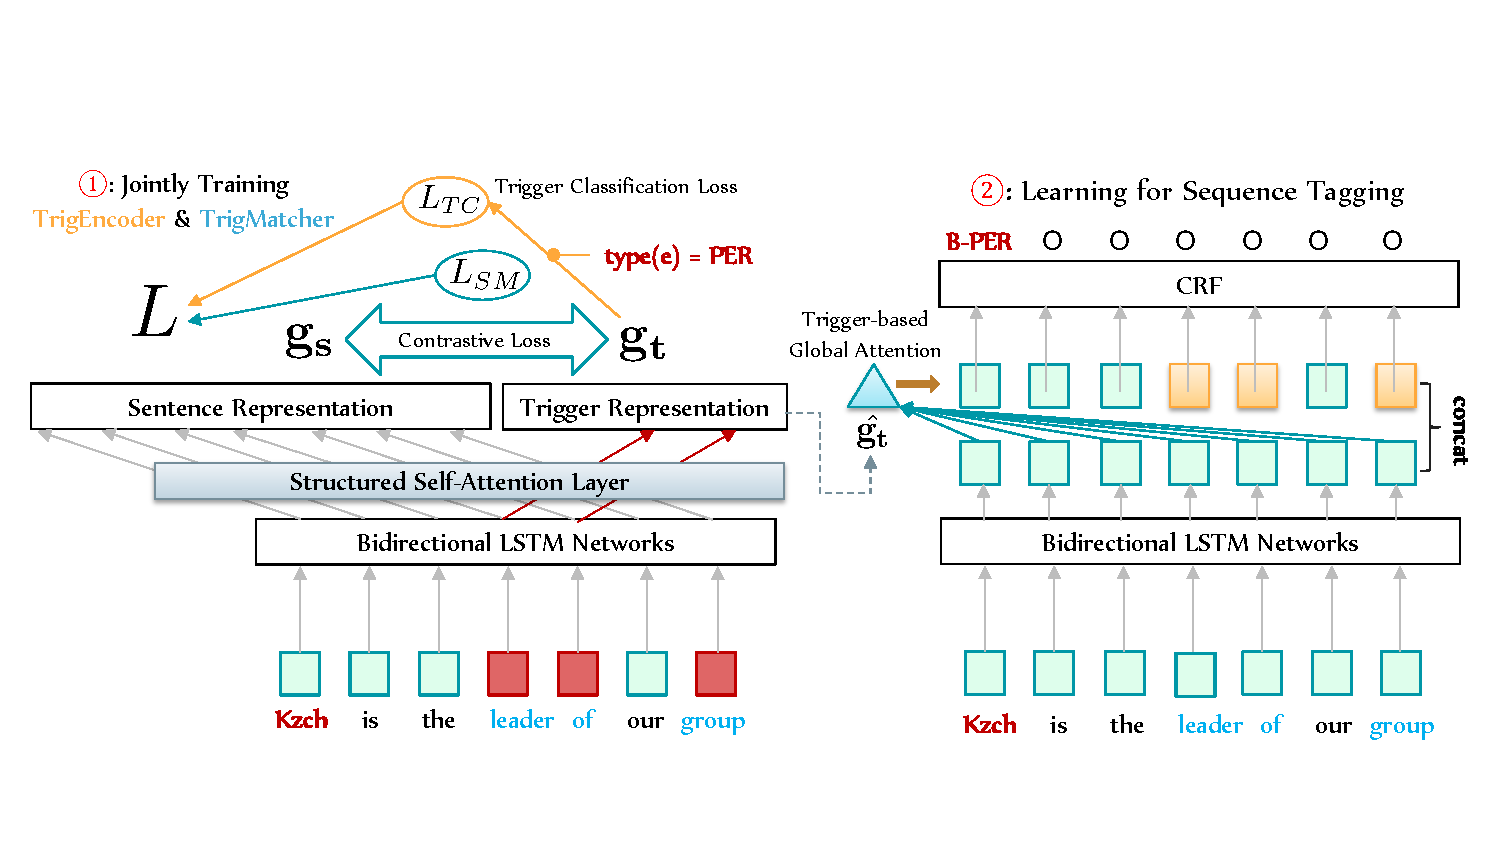
\includegraphics[width=0.85\linewidth]{LatexDiss/figures/tmn.pdf}
	\caption{Two-stage training of the \textit{Trigger Matching Network}. We first jointly train the {\texttt{TrigEncoder}} (via trigger classification) and the \texttt{TrigMatcher} (via contrastive loss). Then, we reuse the training data trigger vectors as attention queries in the \texttt{SeqTagger}.} 
	\label{fig:framework}
\end{figure*}

Learning trigger representations and semantically matching them with sentences are inseparable tasks.
Desired trigger vectors capture the semantics in a shared embedding space with token hidden states such that sentences and triggers can be semantically matched.
Learning an attention-based matching module between entity triggers and sentences is necessary so that triggers and sentences can be semantically matched.
Therefore, as the first learning stage, we propose to jointly train the trigger encoder (\texttt{TrigEncoder}) and the attention-based trigger matching module (\texttt{TrigMatcher}) using a shared embedding space.

Specifically,
for a sentence $\mathbf{x}$ with multiple entities $\{e_1, e_2,\cdots\}$, for each entity $e_i$ we assume that there is a set of triggers $T_i=\{t^{(i)}_1, t^{(i)}_2, \cdots\}$.
To enable more efficient batch-based training, we reform the trigger-based annotated dataset $\mathcal{D}_{T}$ such that each new sequence contains only one entity and one trigger.
We then create a training instance by pairing each entity with one of its triggers, denoted $(\mathbf{x}, e_i, t^{(i)}_j)$.
The learning objective in this stage is to output the tag sequence $\mathbf{y}$. %TODO is this still the learning objective? Isn't the learning objective here the trigger classification loss and contrastive loss?


For each reformed training instance $(\mathbf{x}, e, t)$, we first apply a bidirectional LSTM (BLSTM) on the sequence of word vectors\footnote{Here, by ``word vectors'' we mean the concatenation of external GloVe~\citep{Pennington2014GloveGV} word embeddings and char-level word representations from a trainable CNN network~\citep{DBLP:conf/acl/MaH16}.} 
of $\mathbf{x}$, obtaining a sequence of hidden states that are the contextualized word representations $\mathbf{h}_i$ for each token $x_i$ in the sentence. 
We use $\mathbf{H}$ to denote the matrix containing the hidden vectors of all of the tokens, and we use $\mathbf{Z}$ to denote the matrix containing the hidden vectors of all of the trigger tokens inside the trigger $t$.

In order to learn a attention-based
representation of both triggers and sentences, we follow the self-attention method introduced by ~\cite{selfattentive} and described in Sec~\ref{sec:ourframework} as follows:
{
{
		\begin{align*} 
			\vec{a}_{sent}&=\operatorname{SoftMax}\left(W_{2} \tanh \left(W_{1} \mathbf{H}^{T}\right)\right)\\
			\mathbf{g_s}&=\vec{a}_{sent}\mathbf{H}\\
			\vec{a}_{trig}&=\operatorname{SoftMax}\left(W_{2} \tanh \left(W_{1} \mathbf{Z}^{T}\right)\right)\\
			\mathbf{g_t}&=\vec{a}_{trig}\mathbf{Z}
		\end{align*} 
	}
}  
Here, $W_1$ and $W_2$ are two trainable parameters for computing self-attention score vectors $\vec{a}_{sent}$ and $\vec{a}_{trig}$, essentially the level of importance the self-attention layer has given to each token.
We obtain a vector representing the weighted sum of the token vectors in the entire sentence as the final sentence vector $\mathbf{g_s}$. Similarly, $\mathbf{g_t}$ is the final trigger vector, representing the weighted sum of the token vectors in the trigger.

We want to use the type of the associated entity as supervision to guide the trigger representation.
Thus, the trigger vector $\mathbf{g_t}$ is further fed into a multi-class classifier to predict the \textit{type} of the associated entity $e$ (such as \texttt{PER}, \texttt{LOC}, etc) which we use $\texttt{type}(e)$ to denote. Because our model is a multi-class classifier (selecting which label should be assigned to a given word), we use a cross-entropy loss function.  The loss is low if the model predicts a high probability for the correct label.
The trigger classification loss is as follows, where $\theta_{TC}$ is the learning parameter:
{
	{  
		\begin{align*} 
		L_{TC}=-\sum \log \mathrm{P} \left(\texttt{type}(e)~|~ \mathbf{g_t}; \theta_{TC}\right) 
		\end{align*} 
	}
}  
In order to learn to match triggers and sentences based on their self-attention-based representations, we use contrastive loss \citep{hadsell2006dimensionality}. 
Contrastive loss is a loss method for unlabeled data depending on both positive examples (a pair of vectors of the same class) and negative examples (a pair of vectors of different classes). The contrastive loss is low if the positive examples have a small distance between their two vectors and the negative examples have a large distance between their two vectors. This ensures that vectors of the same class are encoded near each other in the vector space.

The intuition behind our use of contrastive loss is that a trigger and the sentence that the trigger belongs to should have similar representations (i.e. have a small distance betweeen them, $d$).
\texttt{TrigMatcher} needs to be trained with both positive and negative examples of the form (sentence, trigger, label), so we randomly mix the triggers and sentences so that we have negative examples (i.e. mismatches). 
For the negative examples, we expect a margin $m$ between their representations. 
The contrastive loss of the soft matching is defined as follows, where $\mathds{1}_{\text{matched}}$ is $1$ if the trigger belongs to this sentence and $0$ if they are mismatched:
{
	{
		\begin{align*}  
		d&=\left\|\mathbf{g_s}-\mathbf{g_t}\right\|_{2}\\
			L_{SM} = (1-\mathds{1}_{\text{matched}}) &\frac{1}{2}\left(d\right)^{2}+\mathds{1}_{\text{matched}} \frac{1}{2}\left\{\max \left(0, m-d\right)\right\}^{2}
		\end{align*} 
	}
}  

Thus, the joint loss we aim to optimize is $L = L_{TC} + \lambda L_{SM}$.



\subsection{Trigger-Enhanced Sequence Tagging for NER}
\label{sec:secondstage}
Following the most common design of neural NER architecture, BLSTM-CRF \citep{DBLP:conf/acl/MaH16}, we incorporate the entity triggers as attention queries (explained in Sec~\ref{sec:ourframework})
to train a trigger-enhanced sequence tagger for NER. Note that the BLSTM used in the the \texttt{TrigEncoder} and \texttt{TrigMatcher} modules is the same BLSTM we use in the \texttt{SeqTagger} to obtain $\mathbf{H}$, the matrix containing the hidden vectors of all of the tokens.
Given a sentence $\mathbf{x}$, we use the previously trained \texttt{TrigMatcher} to compute the mean of all the trigger vectors $\hat{\mathbf{g_t}}$ associated with this sentence.
Following the conventional attention method~\citep{luong2015effective}, 
we incorporate the mean trigger vector as the query, creating a sequence of attention-based token representations, $\mathbf{H}'$.
{
    {
        \begin{align*} 
            \vec{\alpha}  &= \operatorname{SoftMax}\left(\boldsymbol{v}^{\top} \tanh \left({U}_{1}\mathbf{H}^T + {U}_{2}\hat{\mathbf{g_t}}^T \right)^{\top}\right)\\
            \mathbf{H'} &=  \vec{\alpha}~\mathbf{H}
        \end{align*} 
    }
}
\noindent
where $U_1$, $U_2$, and $v$ are trainable parameters for computing the trigger-enhanced attention scores for each token.
Finally, we concatenate the original token representation $\mathbf{H}$ with the trigger-enhanced one $\mathbf{H}'$ as the input ($[\mathbf{H};\mathbf{H}']$) to the final CRF tagger.
Note that in this stage, our learning objective is the same as conventional NER, which is to correctly predict the tag for each token.




\subsection{Inference on Unlabeled Sentences}
\label{sec:inference}

When inferencing tags on unlabeled sentences,
we do not know the sentence's triggers.
Instead, we use the \texttt{TrigMatcher} to compute the similarities between the self-attended sentence representations and the trigger representations, using the most suitable triggers as additional inputs to the \texttt{SeqTagger}.
Specifically, we have a trigger dictionary from our training data, $\mathcal{T}=\{t | (\cdot, \cdot, t) \in \mathcal{D}_T\}$.
Recall that we have learned a trigger vector for each of them, and we can load these trigger vectors as a look-up table in memory.
For each unlabeled sentence $\mathbf{x}$, we first compute its self-attended vector $\mathbf{g_s}$ as we do when training the \texttt{TrigMatcher}.
Using L2-norm distances to compute the contrastive loss, we efficiently retrieve the most similar triggers in the shared embedding space of the sentence and trigger vectors.
Then, we calculate $\hat{\mathbf{g_t}}$, the mean of the top $k$ nearest semantically matched triggers, and use it as the attention query for \texttt{SeqTagger}, as we did in Section~\ref{sec:secondstage}.
Now, we can produce trigger-enhanced sequence predictions on unlabeled sentences, as shown in \figref{fig:inference}.

\begin{figure*}[h]
 	\centering 
% \hspace{-15pt}
	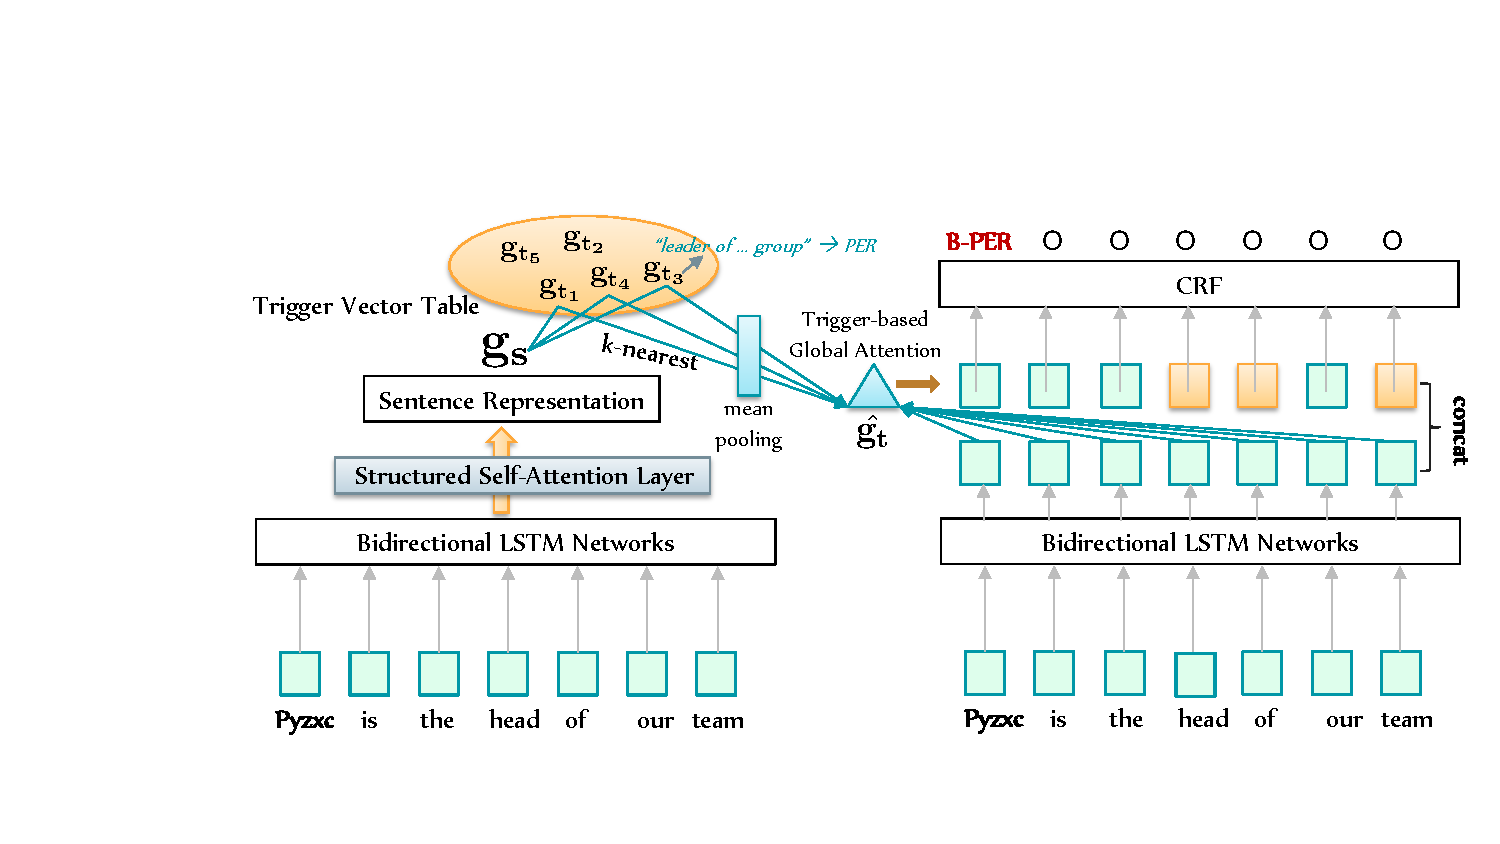
\includegraphics[width=0.85\linewidth]{LatexDiss/figures/inference.pdf}
	\caption{The \textit{inference} process of the TMN framework. It uses the \texttt{TrigMatcher} to retrieve the k nearest triggers and average their trigger vectors as the attention query for the previously trained \texttt{SeqTagger}. This is how a previously unseen cue phrase (e.g., \textit{``head of ... team''}) can be matched with a previously seen trigger (e.g., \textit{``leader of ... group''}).} 
	\label{fig:inference}
\end{figure*}






\section{Experiments}
\label{sec:exp}
This section discusses how we collected entity triggers and empirically studies the data-efficiency of our framework.
\subsection{Annotating Triggers as Explanatory Supervision}
\label{sec:trigger}

\begin{figure*}[h] % TODO: Trigger 1 instead of Trigger !
	\centering
% 	\hspace*{-.2in}
	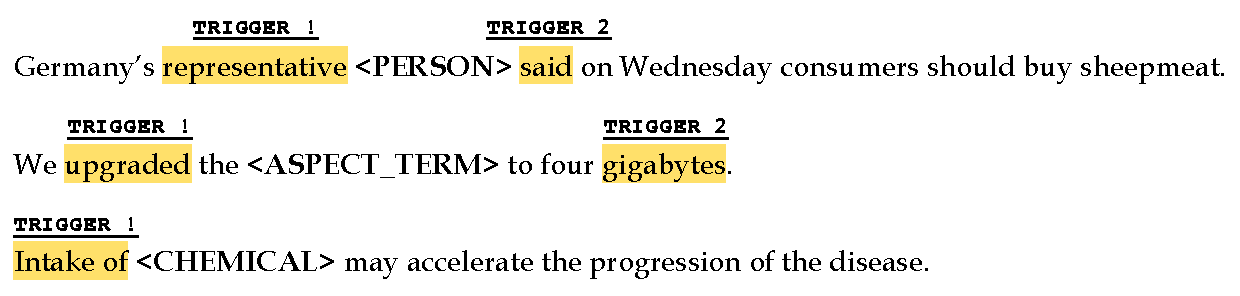
\includegraphics[width=0.9\linewidth]{LatexDiss/figures/triggers.pdf}
	\caption{Example of trigger annotations.}
% 	\vspace{-15pt}
	\label{fig:triggerannotation}
\end{figure*}

We used a general domain dataset CoNLL2003~\citep{conll} and a bio-medical domain dataset BC5CDR~\citep{bc5cdr}.
Both datasets are well-studied and popular in evaluating the performance of neural named entity recognition models such as BLSTM-CRF~\citep{DBLP:conf/acl/MaH16}.
In order to collect the entity triggers from human annotators, 
we used \textit{Amazon SageMaker}\footnote{An advanced version of \textit{Amazon Mechanical Turk}. \url{https://aws.amazon.com/sagemaker/}} to crowd-source entity triggers.
Specifically, we sampled 20\% of each training set and reformed the data to reflect the entity $+$ entity trigger format that we discussed in Section~\ref{sec:problem}.
Annotators were asked to annotate a group of words that would be helpful in typing and/or detecting the occurrence of a particular entity in the sentence.
We masked the entity tokens with their types so that human annotators were more focused on the non-entity words in the sentence when considering the triggers.
For annotators' convenience, we separated a sentence with multiple entities into single-entity sentences and masked the entity word into its corresponding entity type. Figure~\ref{fig:triggerannotation} demonstrates the annotator's interface.
In the end, we consolidate multiple triggers for each entity by taking the intersection of the three annotators' results. 
Statistics of the final curated triggers are summarized in Table~\ref{tab:numtrig}.
We released the 14k entity triggers to the community for future research in trigger-enhanced NER learning. % TODO footnote to URL

\begin{table*}[h]
	\begin{singlespace}
	\centering
	\scalebox{0.7
	}{
		\begin{tabular}{@{}lcccccccc@{}}
			\toprule   
			\textbf{Dataset} &      
			\multicolumn{1}{C{.2\textwidth}}{Entity Type}  &  
			\multicolumn{1}{C{.2\textwidth}}{\# Entities} & 
			\multicolumn{1}{C{.2\textwidth}}{\# Triggers} & 
			\multicolumn{1}{C{.2\textwidth}}{Avg. \# Triggers per Entity} & 
			\multicolumn{1}{C{.2\textwidth}}{Avg. Trigger length} 
			\\ 
			\midrule
			\textsc{CONLL 2003} & \textsc{PER} & 1,608 & 3,445 & 2.14 & 1.41 \\
			& \textsc{ORG} & 958 & 1,970 & 2.05 & 1.46 \\  
			& \textsc{MISC} & 787 & 2,057 & 2.61 & 1.4 \\ 
		    & \textsc{LOC} & 1,781 & 3,456 & 1.94 & 1.44 \\ 
		    \midrule
			& \textbf{Total} & 5,134 & 10,938 & 2.13 & 1.43\\ 
			\midrule\midrule
			\textsc{BC5CDR} & \textsc{Disease} & 906 & 2,130 & 2.35 & 2.00  \\
			& \textsc{Chemical} & 1,085 & 1,640 & 1.51 & 1.99  \\ 
			\midrule
			& \textbf{Total} & 1,991 & 3,770 & 1.89 & 2.00 \\ 
			\bottomrule
		\end{tabular}
	} 
	\caption{Statistics of the crowd-sourced entity triggers.} \label{tab:numtrig}
	\end{singlespace}
\end{table*}


\subsection{Base model}
We required a base model to compare with our proposed TMN model in order to validate whether the TMN model effectively uses triggers to improve model performance in a limited label setting.
We chose the CNN-BLSTM-CRF~\citep{DBLP:conf/acl/MaH16} as our base model for its wide usage in the research of neural NER model.
Our TMNs are implemented within the same codebase and use the same external word vectors from GloVE~\citep{Pennington2014GloveGV}. The hyper-parameters of the CNNs, BLSTMs, and CRFs are also the same.
This ensures a fair comparison between a typical non-trigger NER model and our trigger-enhanced framework.

% We apply semi-supervised methods to two categories of datasets: 1) datasets with hard-matched triggers and 2) datasets with soft-matched triggers. 
% We use several semi-supervised methods: (1) Self-Training ~\citep{Rosenberg2005SemiSupervisedSO} iteratively expands the labeled set with the most confident predictions from the unlabeled set during training.
% (2) Pseudo-Labeling ~\citep{lee2013pseudo} first trains the model on labeled dataset, and generate pseudo labels for unlabeled data using the model by selecting the label with maximum predicted probability. Then, it trains with both labeled dataset and pseudo-labels. In this method, we create pseudo-labels with matched sentences.

\subsection{Results and analysis}
We experimented with using different proportions of the training data for both the base model and the TMN.
From Table~\ref{tab:results}, we see that the TMN models using 20\% of the training sentences with annotated triggers achieves comparable results to the BLST-CRF models using 50\% (BC5CDR)$\sim$70\% (CONLL03) of the training data.
Even though the annotators spent slightly more effort per sentence when tagging triggers, the drastic improvement in model performance evidences the merit of our approach.
With the self-training method~\citep{Rosenberg2005SemiSupervisedSO}, which iteratively expands the labeled set with the most confident predictions from the unlabeled set during training, we further improve the TMN model's F1 scores by about 0.5$\sim$1\%. 

\begin{table*}[h]
% \vspace{-0.3cm}
	\centering
	\scalebox{0.7}
	{
	    \begin{singlespace}
		\begin{tabular}{@{}>{\columncolor{LightCyan}}c|ccc|>{\columncolor{LightCyan}}c|ccc|cccc@{}}
			\toprule
			\multicolumn{11}{c}{\textbf{CONLL 2003}}\\
			\toprule
			\rowcolor{white} & 
			\multicolumn{3}{c|}{\textsc{BLSTM-CRF}}  & 
			&
			\multicolumn{3}{c|}{\textsc{TMN}}  &  
			\multicolumn{3}{c}{\textsc{TMN + self-training}}  
			\\
			\midrule
			\rowcolor{white}\textbf{ent.}  &
			\multicolumn{1}{c}{Precision}  &    
			\multicolumn{1}{c}{Recall}  &
			\multicolumn{1}{c|}{F1}  &  
			\textbf{trig. } &
			\multicolumn{1}{c}{Precision}  &    
			\multicolumn{1}{c}{Recall}  &
			\multicolumn{1}{c|}{F1} &
			\multicolumn{1}{c}{Precision}  &    
			\multicolumn{1}{c}{Recall}  &
			\multicolumn{1}{c}{F1}  & 
			\\ 
			\midrule 
			5\%  &  70.85 & 67.32 & 69.04 & 3\%  & 76.36 & 74.33 & 75.33 & 80.36 & 75.18 & 77.68 \\
			10\% &  76.57 & 77.09 & 76.83 & 5\%  & 81.28 & 79.16 & 80.2  & 81.96 & 81.18 & 81.57   \\
            20\% &  82.17 & 80.35 & 81.3  & 7\%  & 82.93 & 81.13 & 82.02 & 82.92 & 81.94 & 82.43   \\
            30\% &  83.71 & 82.76 & 83.23 & 10\% & 84.47 & 82.61 & 83.53 & 84.47 & 82.61 & 83.53   \\
            40\% &  85.31 & 83.1  & 84.18 & 13\% & 84.76 & 83.69 & 84.22 & 84.64 & 84.01 & 84.33   \\
            50\% &  85.07 & 83.49 & 84.27 & 15\% & 85.61 & 84.45 & 85.03 & 86.53 & 84.26 & 85.38   \\
            60\% &  85.58 & 84.54 & 85.24 & 17\% & 85.25 & 85.46 & 85.36 & 86.42 & 84.63 & 85.52   \\
            \textbf{\underline{70\%}} &  86.87 & 85.3  & \textbf{\underline{86.08}}&\textbf{ 20\% }& 86.04 & 85.98 & \textbf{86.01} & 87.09 & 85.91 & \textbf{86.5 }  \\
			\midrule
			\multicolumn{11}{c}{\textbf{BC5CDR}}\\
			\toprule
			\rowcolor{white} & 
			\multicolumn{3}{c|}{\textsc{BLSTM-CRF}}  & 
			&
			\multicolumn{3}{c|}{\textsc{TMN}}  &  
			\multicolumn{3}{c}{\textsc{TMN + self-training}}  
			\\
			\midrule
			\rowcolor{white}\textbf{ent.}  &
			\multicolumn{1}{c}{Precision}  &    
			\multicolumn{1}{c}{Recall}  &
			\multicolumn{1}{c|}{F1}  &  
			\textbf{trig.}  &
			\multicolumn{1}{c}{Precision}  &    
			\multicolumn{1}{c}{Recall}  &
			\multicolumn{1}{c|}{F1} &
			\multicolumn{1}{c}{Precision}  &    
			\multicolumn{1}{c}{Recall}  &
			\multicolumn{1}{c}{F1}  & 
			\\ 
			\midrule 
			5\%  &  63.37 & 43.23 & 51.39 & 3\%  & 66.47 & 57.11 & 61.44 & 65.23 & 59.18 & 62.06 \\
			10\% &  68.83 & 60.37 & 64.32 & 5\%  & 69.17 & 73.31 & 66.11 & 68.02 & 66.76 & 67.38   \\
            20\% &  79.09 & 62.66 & 69.92 & 7\%  & 64.81 & 69.82 & 67.22 & 69.87 & 66.03 & 67.9   \\
            30\% &  80.13 & 65.3 & 71.87 & 10\% & 71.89 & 69.57 & 70.71 & 69.75 & 72.75 & 71.22   \\
            40\% &  82.05 & 65.5 & 72.71 & 13\% & 73.36 & 70.44 & 71.87 & 75.11 & 69.31 & 72.1   \\
            \textbf{\underline{50\%} }&  82.56 & 66.58 & \textbf{\underline{73.71}} & 15\% & 70.91 & 72.89 & 71.89 & 71.23 & 73.31 & 72.26  \\
            60\% &  81.73 & 70.74 & 75.84 & 17\% & 75.67 & 70.6 & 73.05 & 77.47 & 70.47 & 73.97   \\
            70\% &  81.16 & 75.29 & 76.12 & \textbf{20\% }& 77.47 & 70.47 & \textbf{73.97} & 75.23 & 73.83 & \textbf{74.52}   \\
			\midrule
			\bottomrule
		\end{tabular}
		\end{singlespace}
	}
	\caption{Labor-efficiency study on BLSTM-CRF and TMN. ``ent.'' means the percentage of the sentences (labeled only with entity tags) we used for BLSTM-CRF, while ``trig.'' denotes the percentage of the sentences (labeled with both entity tags and trigger tags) we used for TMN. }
	\label{tab:results}
\end{table*}

\begin{figure}[h]
\centering
	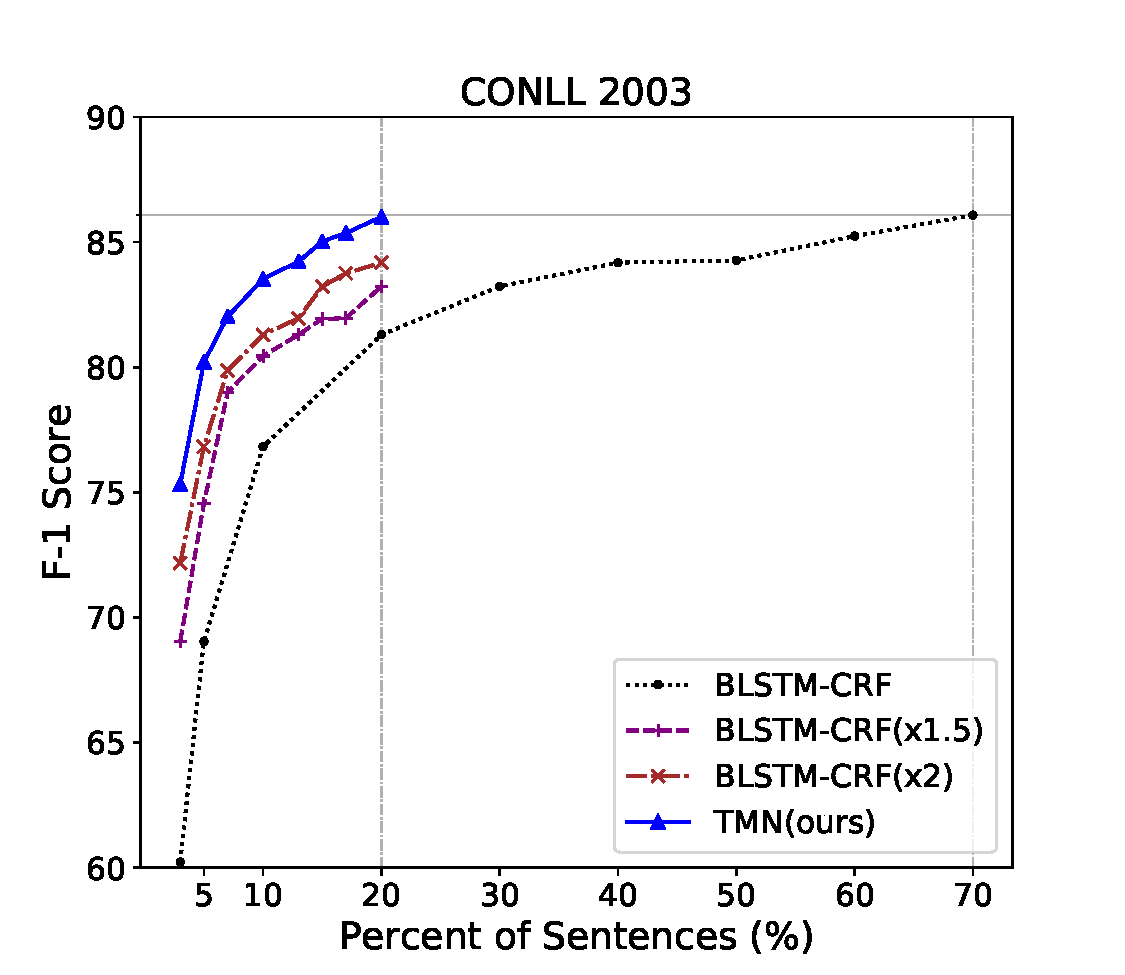
\includegraphics[width=0.8\linewidth]{LatexDiss/figures/singlelabelefficiency.pdf}
	\caption{ The cost-effectiveness study. We stretch the curve of the BLSTM-CRF parallel to the x-axis by 1.5 and 2 respectively. Even if we assume annotating  entity triggers cost 150/200\% the amount of human effort as annotating entities only, TMN is still much more effective. }
	\label{fig:curve}
\end{figure}

Although it is hard to accurately study the time cost on the crowd-sourcing platform we used\footnote{Annotators may suspend jobs and resume them without interaction with the crowd-sourcing platform.}, based on our offline simulation we argue that annotating both triggers and entities are about $1.5$ times (``BLSTM-CRF (x1.5)'') longer than only annotating entities.
In \figref{fig:curve}, The x-axis for BLSTM-CRF reflects the number of sentences annotated with only entities, while for TMN it means the number of sentences tagged with both entities and triggers. 
In order to reflect human annotators spending 1.5 to 2 times as long annotating triggers and entities as they spend annotating only entities, we stretch the x-axis for BLSTM-CRF. For example, the line labeled (``BLSTM-CRF (x2)'') associates the actual F1 score for the model trained on 40\% of the sentences with the x-axis value of 20\%. 
We can clearly see that the proposed TMN outperforms the BLSTM-CRF model by a large margin. 
Even if we consider the extreme case that tagging triggers requires twice the human effort (``BLSTM-CRF (x2)''), the TMN is still significantly more labor-efficient in terms of F1 scores. Based on these results, we claim that 1) when annotating data from scratch, it is more effective to ask annotators to label both entities and \textit{triggers}, and 2) if entity annotations already exist for some datasets, annotating \textit{triggers} can still boost model performance.


\figref{fig:casestudy} shows two examples illustrating that the trigger attention scores help the TMN model recognize entities. The training data has `per day' as a trigger phrase for chemical-type entities, and this trigger matches the phrase `once daily' in an unseen sentence during the inference phase of \texttt{TrigMatcher}.
Similarly, in CoNLL03 the training data trigger phrase `said it' matches with the phrase `was quoted as saying' in an unlabeled sentence.
These results not only support our argument that trigger-enhanced models such as TMN can effectively learn, but they also demonstrate that trigger-enhanced models can provide reasonable interpretation, something that lacks in other neural NER models.


\begin{figure*}[h]
	\centering 
	% \hspace{-15pt}
	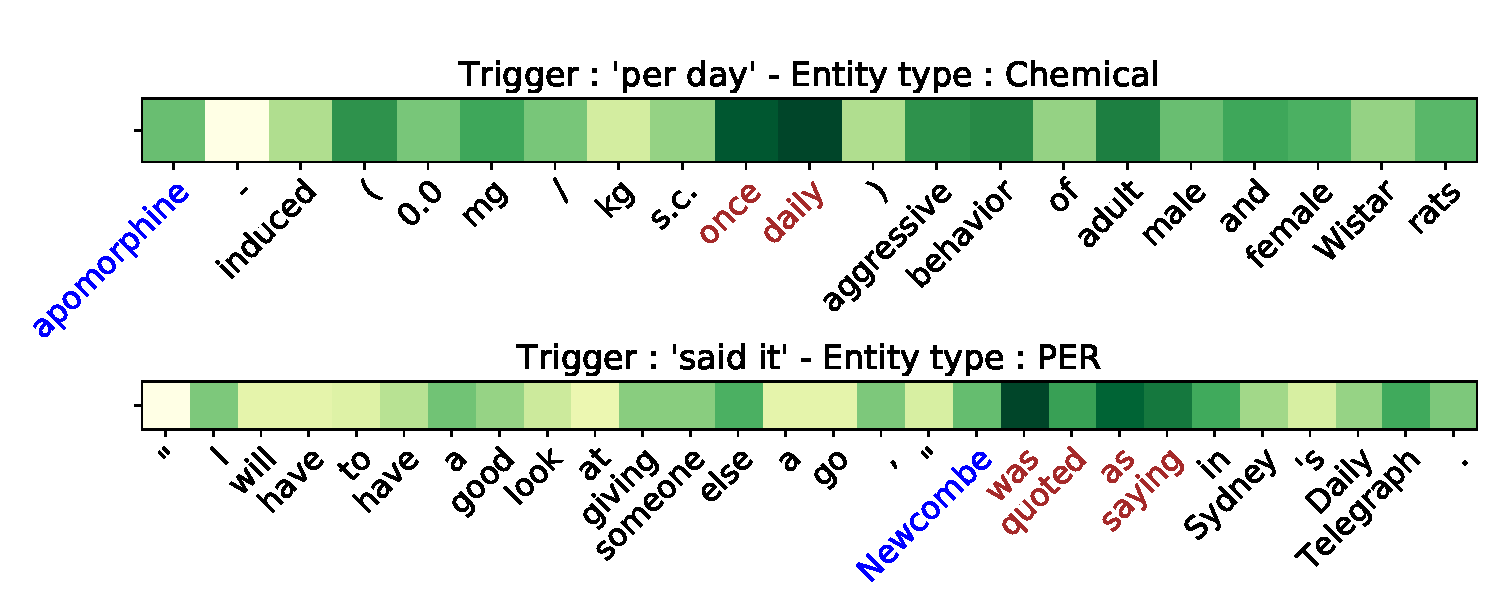
\includegraphics[width=0.7\linewidth]{LatexDiss/figures/casestudy.pdf}
	\caption{Two case studies of the trigger attention scores during inference. The darker cells have higher attention weights.} 
	\label{fig:casestudy}
\end{figure*}


% TODO: add in baselines with access to hard-matched triggers ?? see below

% \paragraph{Supervised learning} First section of ~\tabref{tab:results} shows results in supervised setting. As supervision increases from \textit{triggers}, we expect better results. As shown in ~\tabref{tab:results}, Our results outperform current state-of-the-art NER models.

% \paragraph{Semi-Supervised learning} Second and third section of ~\tabref{tab:results} show results in semi-supervised learning. model training augmentation with soft-matched \textit{triggers} outperforms other baselines with hard-matched \textit{triggers}. It proves that trigger based model training augmentation becomes more powerful when it incorporates with soft matching.


% \begin{figure}[t]
% % 	\centering 
% % \hspace{-50pt}
% 	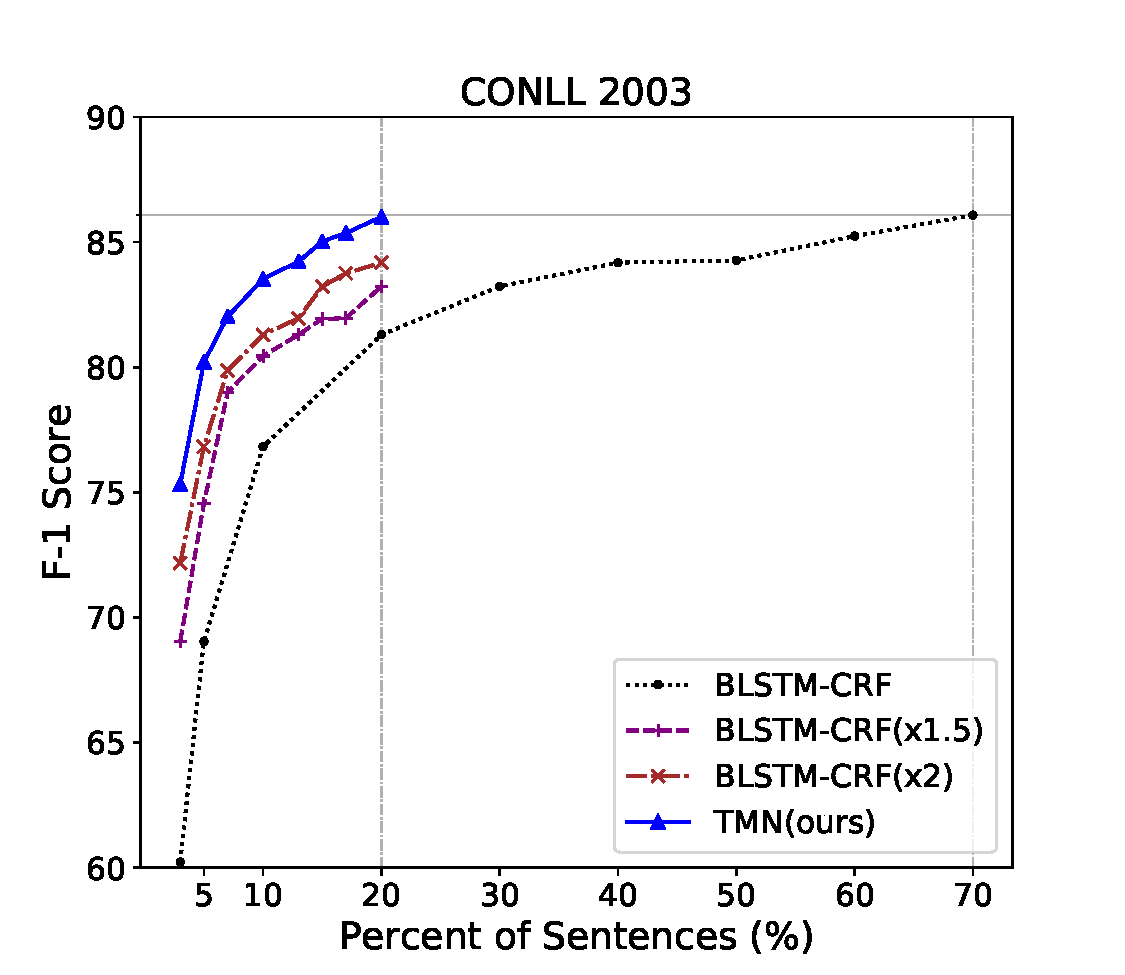
\includegraphics[width=1\linewidth]{LatexDiss/figures/singlelabelefficiency.pdf}
% 	\caption{}
% 	\label{fig:curve}
% \end{figure}


% \paragraph{Label Efficiency} We claim that 1) when annotating data from scratch, it is more effective to ask annotators to label both entities and \textit{triggers}, and 2) if entity annotations already exist for some datasets, annotating \textit{triggers} can also boost model performance. To support the claims, we conduct two experiments demonstrating the label efficiency of our model. First, we sample subsets of the training data (both triggers and entity labels) from 4\% to 20\%. We show the performance of the models trained with different amounts of sampled data. As shown in ~\figref{fig:graph} left, the performance of our model with \textit{trigger} is largely improved when the amount of training data is small.

% Second, we fix the percentage of entity labels into 20\% and vary the amount of trigger labels from 4\% to 20\%. As shown in ~\figref{fig:graph} right, the performance is improved as we have more \textit{triggers}.


\section{Future Directions}
Future research should investigate the use of our framework for trigger-enhanced NER learning in conjunction with related approaches to low-resource learning for NER. 
For example, one could combine dictionary-based distant supervision to our approach by first creating a dictionary using a high-quality corpus. One could also apply active learning by asking human annotators to annotate the triggers chosen by an active sampling algorithm designed for TMN.

Another future direction is to develop highly interpretable NER models using a trigger-enhanced. As was shown in ~\ref{fig:casestudy}, the trigger attention scores during the inference stage can provide reasonable interpretation, meaning that they can be examined to understand ``why'' the model chose its entity predictions. %TODO clarify the use case

It would also be interesting to investigate the possibility of automating entity trigger annotation by developing models to extract novel triggers or by transferring existing entity triggers from one language to low-resource languages.

Finally, I would like to combine the topics of entity triggers and adversarial examples. Since entity triggers can come in a  variety of similar forms (e.g. \textit{had lunch at} versus \textit{ate  dinner  at}), I am interested in perturbing entity triggers from the training data to make the model more robust to variations on entity triggers in the test data.